\documentclass[11pt]{article}
\usepackage{graphicx}
\usepackage{microtype}
\usepackage{newtxtext,newtxmath}
\hbadness 99999
\tolerance=800

\title{	
	\normalfont\normalsize
	\textsc{CS685 -Data Mining}\linebreak
	\medskip 
	\rule{\linewidth}{0.5pt}\linebreak
	\medskip
	{\huge Assignment 1}
	\medskip 
	\rule{\linewidth}{2pt}
}
\author{Shruti Sharma}
\date{Sept 2020}
\begin{document}
\maketitle
It has been long since COVID-19 has launched its attack on us and shocked the world with the consequences that arose because of the pandemic. Analysing the corona cases as they come up helps governments and common people to be cautious about their future plans. They may then decide and form policies for better control over the virus. It will lead to less havoc and lower fatality rate.
\\
Through this assignment, we are expected to follow COVID-19 statistics in India and observe how the pandemic has progressed. Since the death count due to coronavirus is directly dependent on number of confirmed cases at a place, so we concentrate on confirmed, active cases only rather than testing strength or asymptomatic cases.

\section{Data Preprocessing}
COVID-19 data is continuous in nature as the tests are conducted throughout the day all over the country. For a large country like India, getting exact data of a particular date for each state/UT is not an easy task. There were numerous errors like mismatching spellings, missing values, duplicate results, unformatted data etc. \\

The challenge is identifying gaps in data. Considering the scale of rise of cases, absence of data of some places and availability of more data from other places will lead to skewness and wrong insights.

\begin{enumerate}

\item \textit{Mismatching names} - Since there were numerous files over which data was spread out, so uniformity had to be maintained for perfect match of data and prevent loss of information. Such discrepancies were removed manually.

\item \textit{Wrong spellings} - Manual correction of district names was done according to those given on COVID-19 portal.

\item \textit{Missing values} - For datasets including information for 'Unknown', 'Other States', 'Other Regions' and other miscellaneous entries, it was included in the overall data for that particular state's tally. Since no district information was available for some states (eg. Manipur, Assam, Telangana) , so all such districts were combined into one for each state respectively and given the name \textit{ unknown- respective-state-code}. \\ 
Some districts for which no data was available anywhere were eventually discarded from neighbor information.

\item \textit{Unformatted data} - Some states like Delhi, Sikkim were bifurcated into geographical divisions in the provided data although the reporting of cases for them was done cumulatively. For this reason, they had to be concatenated into one.  
\end{enumerate}

\section{Some Particulars}
\begin{enumerate}
\item For weeks/months in which confirmed case count for a district is zero is not shown in the output and should be assumed 0.

\item Data is processed as per data-all.json available on covid19 portal.\\
https://api.covid19india.org/.

\item The required information is extracted from data-all.json and put in data.csv (contains columns that have useful information, rest are omitted.)

\item All outputs are sorted on first column.

\end{enumerate}


\section{Result Analysis}
\begin{enumerate}

\item \textit{Question 1} - The modified neighbours.json was generated as a result of preprocessing described above.

\item \textit{Question 2} - Each district's coronavirus cases were generated in weekly, monthly and overall fashion in the time frame of March-September (1st week).
Through weekly data, it can be seen that with time each district saw a rise in active cases. The first week (in March) had meagre cases. Also data collection was done in an informal manner as most of the districts had missing information for initial weeks. Proper data is recorded from 25th April which led to the more exact analysis from week 7.
\begin{flushleft}
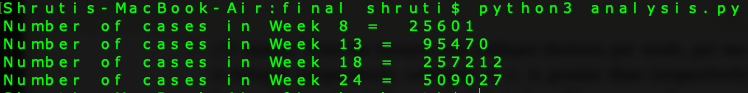
\includegraphics[scale=0.42]{week-cases}
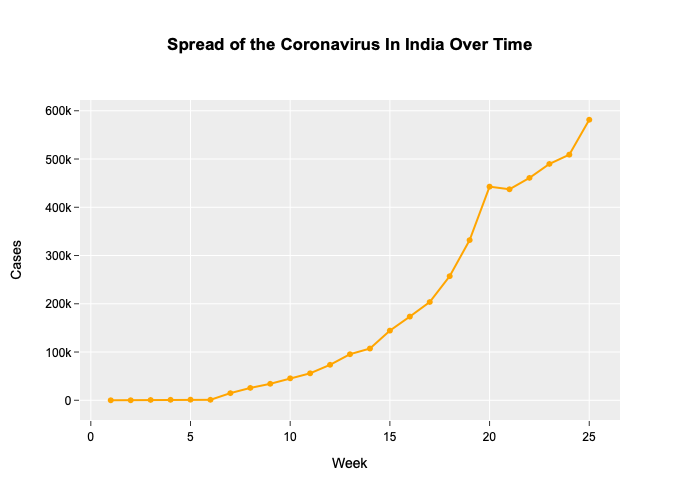
\includegraphics[scale=0.43]{Unknown-2.png}
\end{flushleft}

The monthly variation of cases shows that there has been an exponential rise in the numbers. From just 200 cases in March the number rose to 2 Million in August. \linebreak
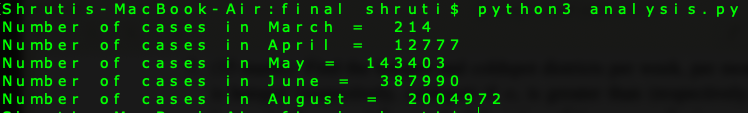
\includegraphics[scale=0.42]{month-cases}

The total number of corona cases in India by 5th Sept are - 

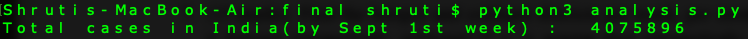
\includegraphics[width=\linewidth]{overall-cases}

\item \textit{Question 3} - The neighbour information was used to deduce an undirected graph in edge list format. Each row of the generated file displays each edge of the graph. This information can be used to capture the effect of neighbours on a district's corona cases by further analysing the actual cases in those districts and their neighbourhood.
Below is the snapshot of how the edge-lists look when plotted. It can be seen there are clusters while some places are well-spaced. Places which are clustered together effect the case-count of all nearby places.
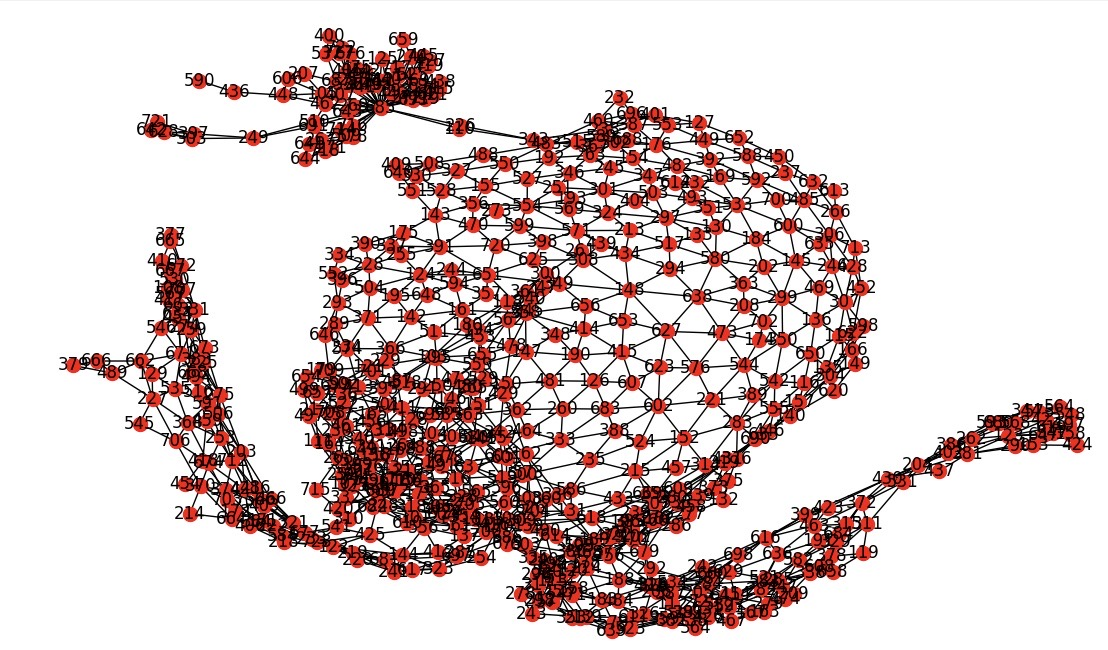
\includegraphics[width=\linewidth]{Figure_1.jpeg}

\item \textit{Question 4} - A kind of cluster analysis is performed by collecting neighbour information and finding mean and standard deviation of a district's cases from its neighbors. This gives information about average cases amongst the neighbors and how dispersed a state's tally is from its neighbors.

\begin{center}
\textit{$ \mu_{A, neighbor} $= Sum of confirmed cases of all of A's neighbors / Number of A's neighbors}
\end{center}

\item \textit{Question 5} - District-level susceptibility is related to viral transmission in districts surrounding it. 

\begin{center}
\textit{$ \mu_{A,state} $= Sum of confirmed cases of all districts in A's state  / (Number of districts in that state - 1)}

\end{center}
\item \textit{Question 6} -  Z-score is a widely used statistical technique used to standardize data to represent the significant changes across the data. Z-score data normalization has been done using the following formula 
\begin{center}
$z$-score = $ \frac{(x_{i} - \mu) }{\sigma} $
\end{center}
Hot spots have statistically significant higher values of $z$-score and cold spots have low values thus signifying the trend of virus' spread.
Normalization has been done to avoid large differences in scale or variance between variables.\\
Highly vulnerable districts are clustered in northern state of Jammu Kashmir, Punjab, Haryana, Uttar Pradesh, West Bengal and Assam. These districts share high population concentration.

\item \textit{Question 7} - Some locations in cold spot regions that have attribute values higher than the overall average while their neighbours' attribute values are lower than the average. Such areas include Nalanda and Siwan districts of Bihar, Korba district in Chhattisgarh, Khordha district in Orissa and Lucknow in Uttar Pradesh. Contrastingly, the hot spot regions derived from the same data show that the attribute values of many districts are lower than the average while their respective neighbours have higher than average attribute values.
 
\item \textit{Question 8} - The most vulnerable districts are Mumbai (Maharashtra), Ahmedabad (Gujarat), Delhi, Chennai (Tamil Nadu) and Bengaluru (Karnataka). The neighborhood hotspots are Bhopal (MP), Assam, Surat (Gujarat)
A significant coldspot is in northern region comprising of Lahual and Spiti and Kullu, eastern regions of Diu and Krishna, also southern Kerala.\\
The more affluent, urban districts that have greater connectivity internationally and are hub of tourist/migrant attractions have higher COVID-19 cases. The states which are densely packed are more vulnerable.

\begin{flushleft}

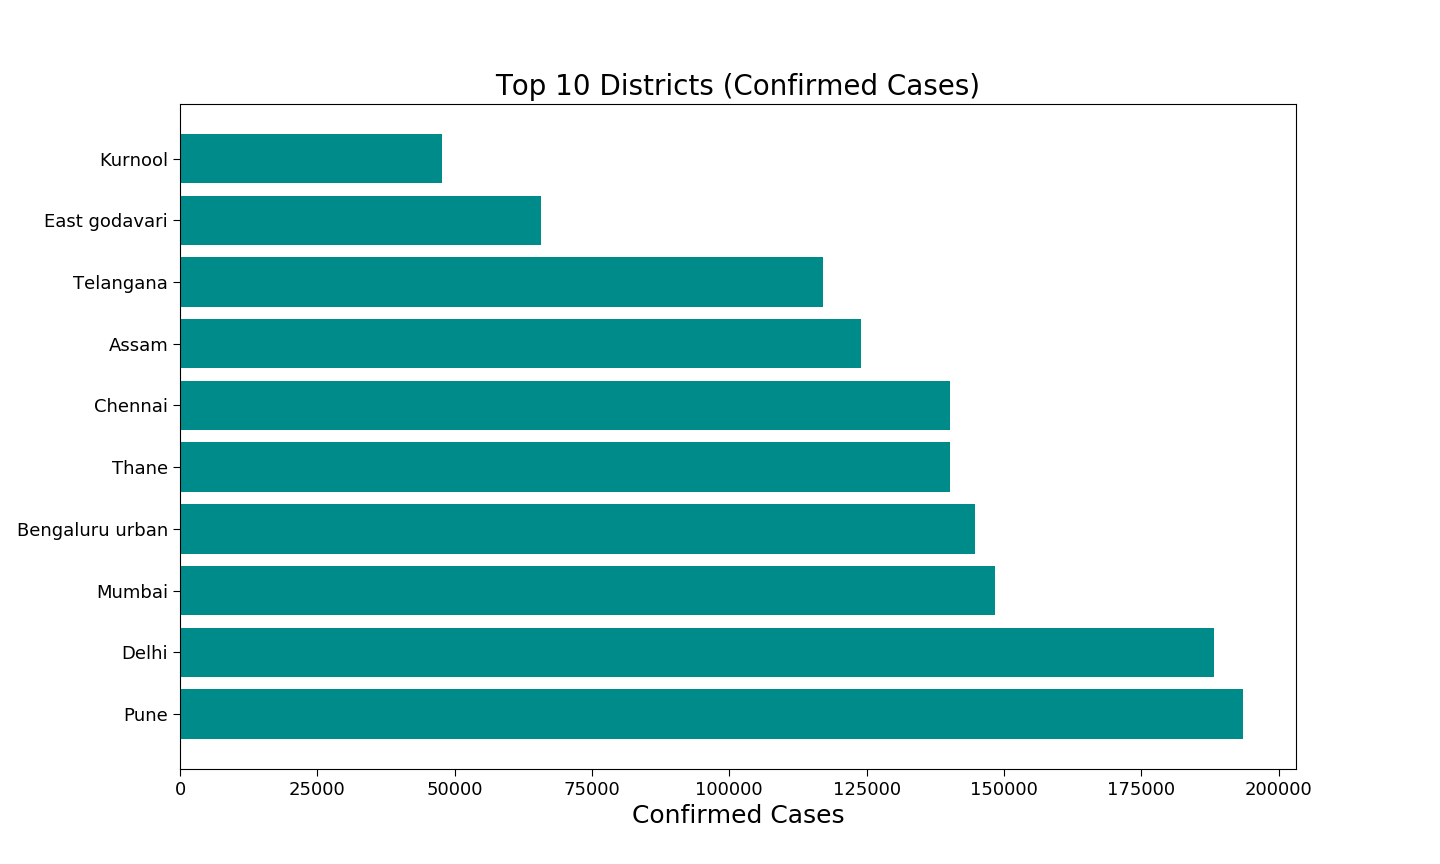
\includegraphics[width=\linewidth]{top-10.png}
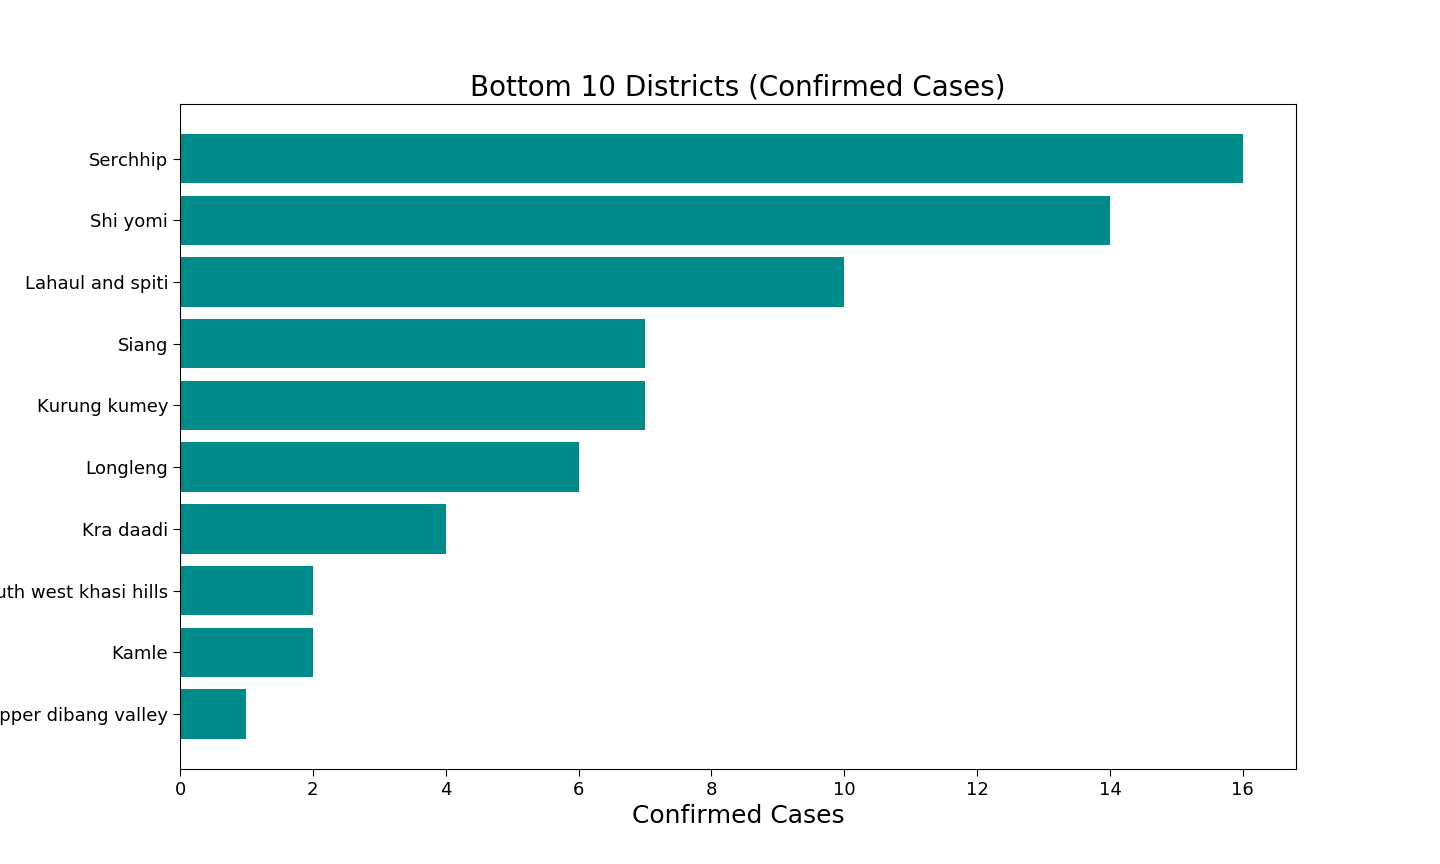
\includegraphics[width=\linewidth]{bot-10.png}
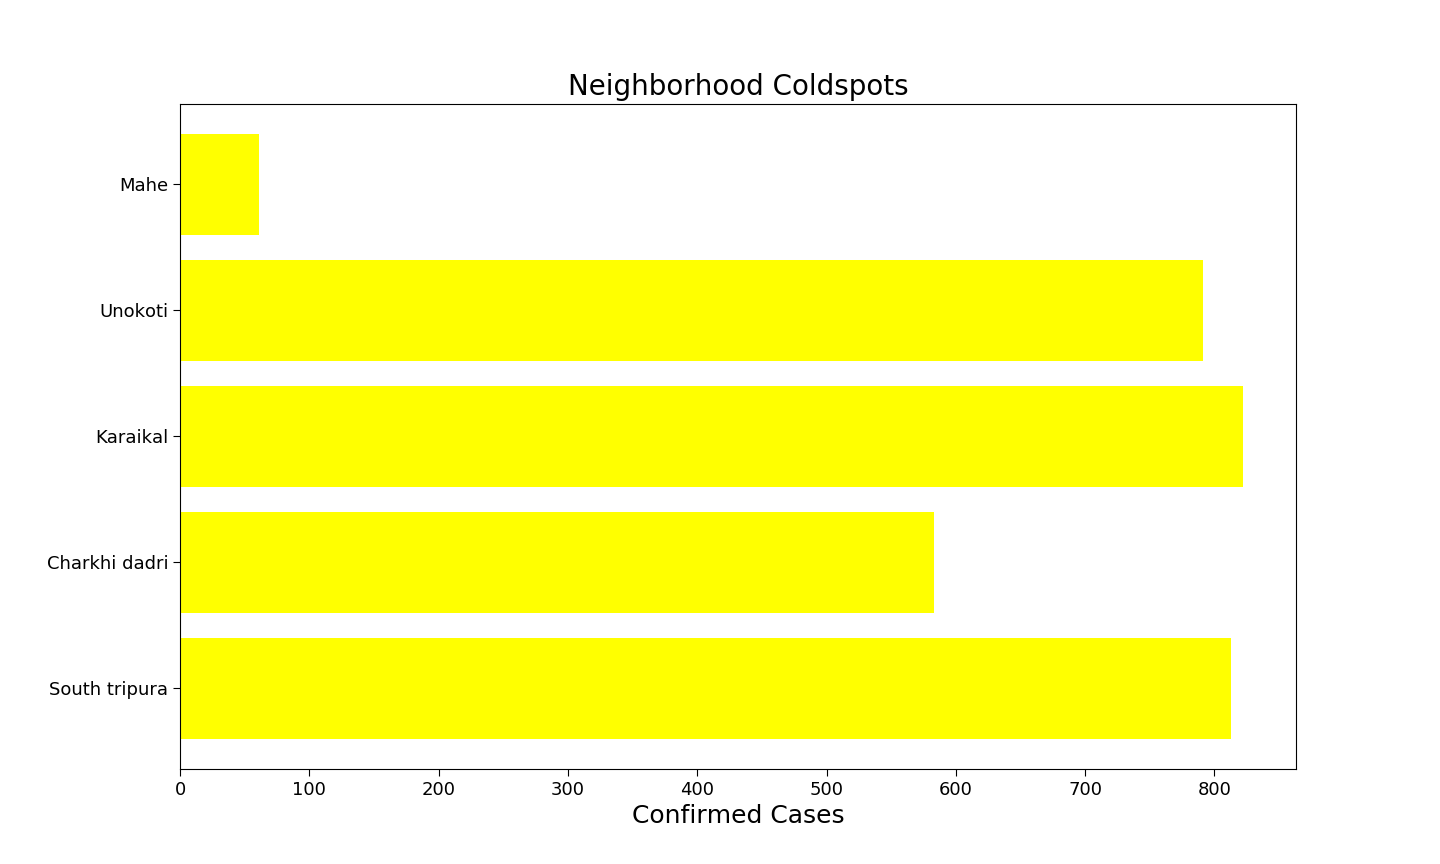
\includegraphics[width=\linewidth]{cold.png}
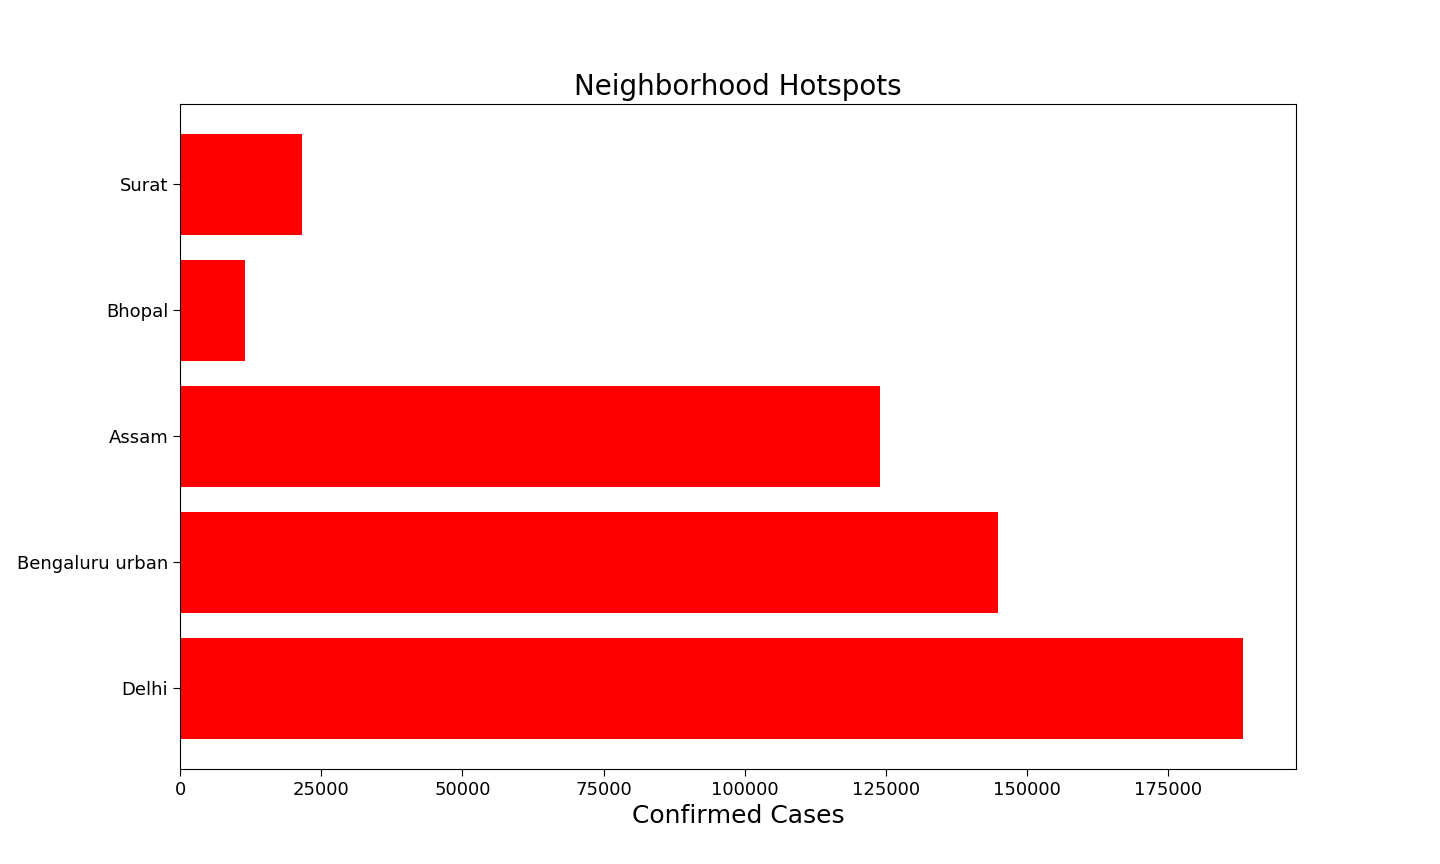
\includegraphics[width=\linewidth]{hot.png}
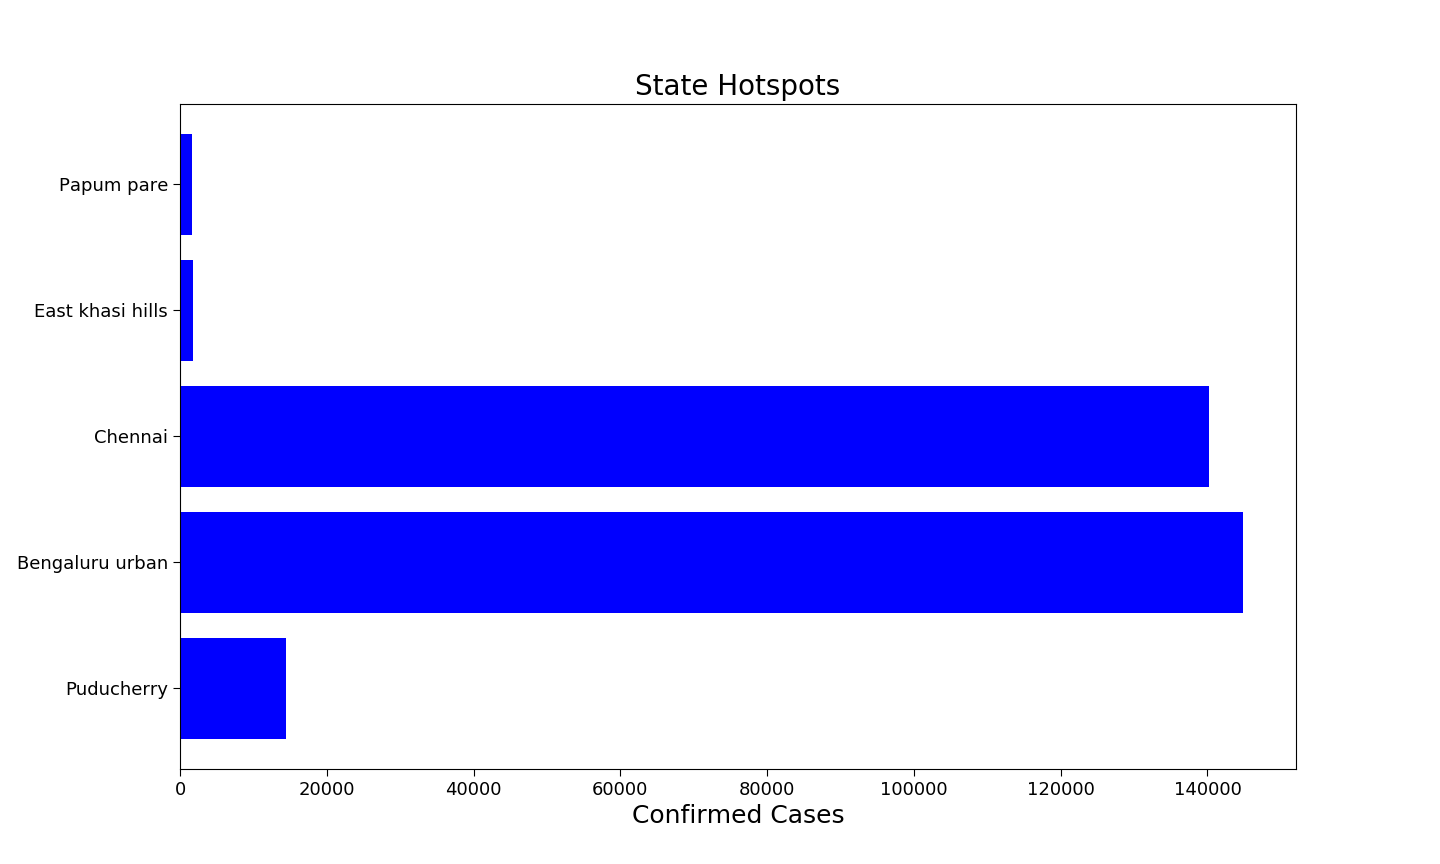
\includegraphics[width=\linewidth]{hot-state.png}

\end{flushleft}

\end{enumerate}

\section{Corrections}

\begin{itemize}
\item \textbf{\textit{Testing Scale}} - The number of confirmed cases at a place had to be normalized with the number of tests carried out at a place. As some places carried out regular tests and others in spurts so for a particular day, the former will have balanced case count while the latter will have high peaks on testing days and a constant count on other days.

\item \textbf{\textit{Population}} -  The amount of tests conducted and the confirmed case count are in every probability connected to the number of people in a particular district. Therefore, the cases had to be normalized with the population too. The actual parameter used should be - Number of confirmed cases per unit population.

\item \textbf{\textit{Under-reporting}} - The extent of under-reporting of confirmed cases by the states.
\end{itemize}

\end{document}